\documentclass{article}%
\usepackage[T1]{fontenc}%
\usepackage[utf8]{inputenc}%
\usepackage{lmodern}%
\usepackage{textcomp}%
\usepackage{lastpage}%
\usepackage{geometry}%
\usepackage{setspace}%
\usepackage{booktabs}%
\usepackage{float}%
\usepackage{graphicx}%
\usepackage{pgfgantt}%
%
\renewcommand{\contentsname}{Summary}%
\usepackage{graphicx}%
\usepackage{fancyhdr}%
\pagestyle{fancy}%
\setlength{\headwidth}{510pt}%
\fancyhead[L]{
\includegraphics[width=2cm]{frigel-logo.png}}%
\fancyhead[C]{\textbf{Project Proposal}}%
\fancyhead[R]{
\includegraphics[width=1cm]{unifi-logo.png}}%
\setlength{\headheight}{2cm}%
%
\begin{document}%
\normalsize%
\newgeometry{top=1cm, bottom=2cm, left=2cm, right=2cm}%
\begin{titlepage}%
\centering%
\vspace*{1cm}%

    \begin{minipage}{0.45\textwidth}
    
\includegraphics[scale=0.5]{frigel-logo.png}
    \end{minipage}
    \hfill
    \begin{minipage}{0.45\textwidth}
    \begin{flushright}
        
\includegraphics[scale=0.1]{unifi-logo.png}
    \end{flushright}
    \end{minipage}
    \\[1.5cm]
    %
\Huge\textbf{Project Proposal}\\[0.5cm]%
\Large\textbf{Automatic Manual Development}\\[2cm]%
\large Romeo Bandinelli, Djonathan Quadras\\%
\large Università degli Studi di Firenze\\[2cm]%
\large April, 2025%
\vfill%
\end{titlepage}%
\newgeometry{top=3.5cm, bottom=2cm, left=2cm, right=2cm}%
\onehalfspacing%
\setlength{\parindent}{12pt}%
\tableofcontents%
\newpage%
\section{About the Project}%
\label{sec:AbouttheProject}%
This project unites Fashion for Future, a University of Florence research lab, and Frigel, a leading manufacturer of cooling and temperature control systems, to develop automated processes for the creation of Frigel's machinery.  The collaboration aims to streamline the currently manual design and development phases, enhancing efficiency and innovation within Frigel's production processes.

%
\subsection{About the Parts}%
\label{subsec:AbouttheParts}%

        This section will present the parts that play a crucial role
        in this project, as well as will describe the responsability
        and duties for each.
        %
\subsubsection{Fashion for Future}%
\label{ssubsec:FashionforFuture}%
The Fashion For Future research lab is a multidisciplinary and multi-skilled environment focused on bridging the gap between academia and industry by connecting technological development with practical application. Within this framework, various events and training sessions are organized to empower fashion sector professionals in the use of artificial intelligence tools. One example is the training GenAI for Designers, that aimed to enhance the design process of new accessories. \\ 
The technical and scientific lead is Prof. Dr. Romeo Bandinelli, Associate Professor in the Department of Industrial Engineering at the University of Florence (Italy) with expertise on management and innovation of industrial processes, with a special focus on the dynamics of product lifecycle management and supply chain operations. He is also a co-founder of Balance, a start-up that supports companies in production planning and continuous improvement initiatives. \\ 
The team also includes the researcher Djonathan Luiz de Oliveira Quadras, who has extensive experience in the textile industry. He has worked on projects involving databases integration, development of managerial dashboards using BI tools, and the application of machine learning and AI for automated data analysis and reporting. Djonathan has also conducted research on the use of AI for production scheduling and maintenance optimization. His current doctoral project focuses on applying AI to fashion supply chains, with an emphasis on data-driven decision-making support for businesses. \\ 

%
\subsubsection{Frigel Group}%
\label{ssubsec:FrigelGroup}%
The Fashion For Future research lab is a multidisciplinary and multi-skilled environment focused on bridging the gap between academia and industry by connecting technological development with practical application. Within this framework, various events and training sessions are organized to empower fashion sector professionals in the use of artificial intelligence tools. One example is the training GenAI for Designers, that aimed to enhance the design process of new accessories. \\ 
The technical and scientific lead is Prof. Dr. Romeo Bandinelli, Associate Professor in the Department of Industrial Engineering at the University of Florence (Italy) with expertise on management and innovation of industrial processes, with a special focus on the dynamics of product lifecycle management and supply chain operations. He is also a co-founder of Balance, a start-up that supports companies in production planning and continuous improvement initiatives. \\ 
The team also includes the researcher Djonathan Luiz de Oliveira Quadras, who has extensive experience in the textile industry. He has worked on projects involving databases integration, development of managerial dashboards using BI tools, and the application of machine learning and AI for automated data analysis and reporting. Djonathan has also conducted research on the use of AI for production scheduling and maintenance optimization. His current doctoral project focuses on applying AI to fashion supply chains, with an emphasis on data-driven decision-making support for businesses. \\ 

%
\newpage%
\section{Proposed Solution}%
\label{sec:ProposedSolution}%
This section proposes an automated solution to streamline the manual generation process, significantly reducing time and resource expenditure while ensuring consistency and accuracy across all documentation.  This automated approach leverages the power of machine learning and large language models to efficiently create comprehensive and user{-}friendly manuals.\newline%
The figure below illustrates the proposed framework.  The process begins with data collection from various internal company sources. This diverse data is then structured and unified within a central database, forming the foundation for the entire system.  This consolidated data is fed into machine learning algorithms to cluster new machines and determine their properties based on information from existing machines.  Finally, these data points and classifications are used by large language models to generate the manual descriptions in clear, understandable language, supporting multiple languages simultaneously. The resulting manual is then automatically exported in the desired format.%


\begin{figure}[h!]%
\centering%
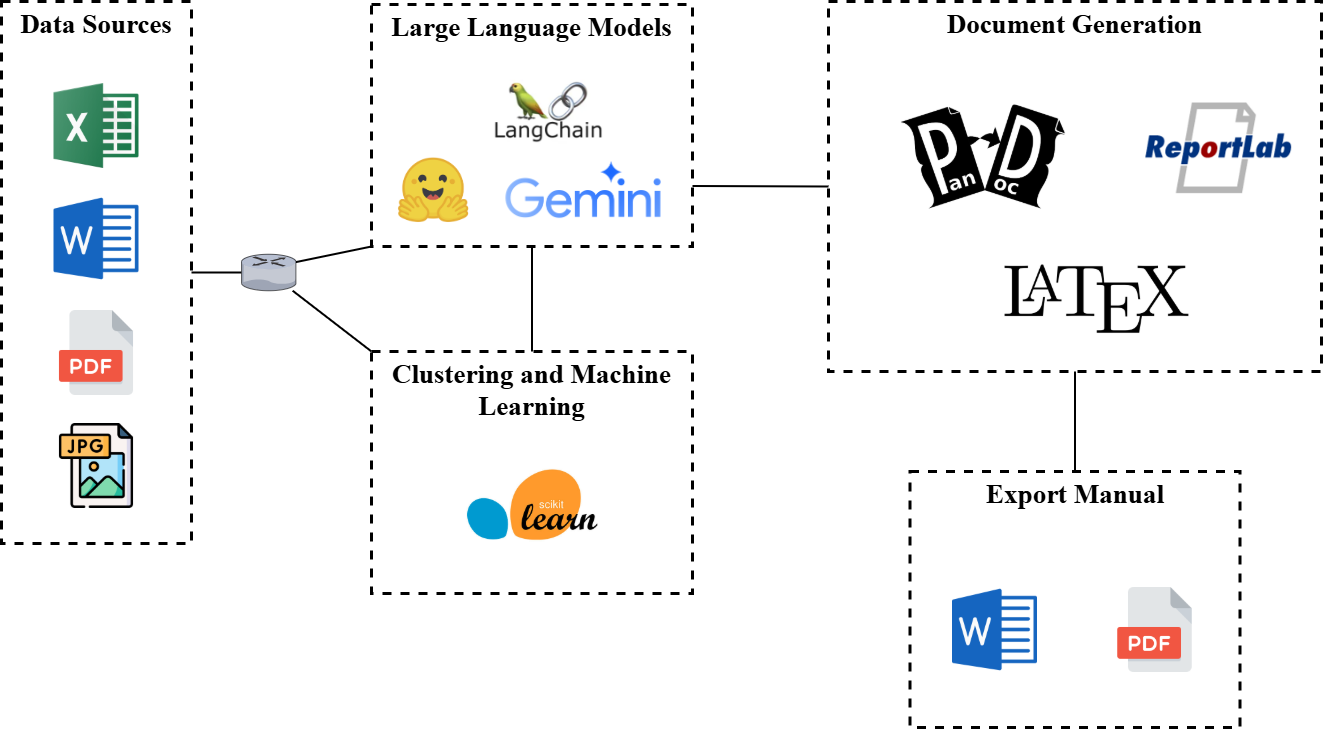
\includegraphics[width=0.8\textwidth]{images/Tools.png}%
\caption{Proposed Framework.}%
\end{figure}

%
\subsection{Data Sources}%
\label{subsec:DataSources}%
Creating comprehensive cooling machine manuals necessitates the compilation of diverse data from multiple sources.  This includes extracting information from the company's Enterprise Resource Planning (ERP) system, integrating engineering team data from Excel spreadsheets, incorporating descriptive text from Word documents, and utilizing diagrams and figures from PDFs detailing previous machine designs and relevant specifications.\newline%
The integration of these varied data sources ensures the manual's accuracy, completeness, and consistency, ultimately providing a user{-}friendly and technically sound guide for operating and maintaining the cooling machine.

%
\subsection{Large Language Models}%
\label{subsec:LargeLanguageModels}%
Large Language Models (LLMs) can significantly automate machine manual generation by processing technical specifications and automatically creating user{-}friendly documentation.  Using LLMs like those accessible through packages such as Langchain, Hugging Face's models, or Google's Gemini, engineers can input data points like component descriptions, operational procedures, and troubleshooting steps, and the LLM can then generate text explaining these in a clear and concise manner, reducing the time and cost associated with manual documentation creation.\newline%
Langchain provides tools to structure and manage the interaction with LLMs, facilitating the process of feeding data and retrieving generated text. Hugging Face offers a wide range of pre{-}trained LLMs readily adaptable for text generation tasks, providing various options for customization and fine{-}tuning. Gemini, a powerful LLM from Google, can directly generate and structure comprehensive documentation from provided data, potentially offering features such as enhanced formatting and automatic indexing.  Each package offers different strengths and interfaces, allowing for flexibility in the development workflow.

%
\subsection{Clustering and Machine Learning}%
\label{subsec:ClusteringandMachineLearning}%
Clustering in machine learning is an unsupervised learning technique that groups data points into clusters based on their similarity.  The goal is to find inherent structure in the data without pre{-}defined labels.  In the context of cooling and temperature control machines, clustering could analyze operational data like power consumption, temperature readings, maintenance records, and error logs.  Machines with similar profiles would be grouped together, revealing patterns like efficient vs. inefficient operation, frequent failure modes in specific machine types, or correlations between environmental conditions and machine performance. This allows for better understanding of machine characteristics, identification of outliers needing attention, and improved predictive maintenance strategies.\newline%
Scikit{-}learn is a popular Python library for machine learning that provides various algorithms for clustering and other data analysis tasks.  For clustering machines based on their operational data, algorithms like K{-}Means, DBSCAN, and hierarchical clustering (e.g., Agglomerative Clustering) could be applied.  The choice of algorithm depends on the data's characteristics (e.g., number of clusters, density, shape of clusters) and the desired outcome of the analysis.  Scikit{-}learn provides tools to evaluate the performance of different clustering algorithms and select the most appropriate one for the specific application.

%
\subsection{Document Generation}%
\label{subsec:DocumentGeneration}%
Generating documents in a specific format and template using Python involves leveraging libraries that handle document structure and formatting.  These libraries allow for programmatic creation of documents, including the incorporation of data, images, and styling according to a predefined template. This is achieved by defining the document's structure, content, and styling within the Python script, which is then processed by the library to generate the final document in the desired format (e.g., PDF, LaTeX, DOCX). For this purpose, packages like Pylatex, ReportLab, and Pandoc can be used.\newline%
Pylatex provides a way to generate LaTeX documents directly from Python code, offering control over LaTeX's extensive formatting capabilities. ReportLab focuses on generating PDF documents, providing a versatile API for creating complex layouts, including tables, images, and text formatting.  Pandoc acts as a universal document converter, allowing Python scripts to generate documents in various formats (like PDF, DOCX, HTML) by leveraging Pandoc's conversion capabilities from a common intermediary format (often Markdown).  Each package offers different strengths; Pylatex excels in LaTeX{-}based documents, ReportLab in PDFs, and Pandoc in its flexibility to handle diverse output formats.

%
\newpage%
\section{Timetable and Activities}%
\label{sec:TimetableandActivities}%

        Here the timetable with the description of the tasks
        to develop the project are included.
        %
\begin{figure}[htbp]%
\centering%

        \begin{ganttchart}{0}{17}
        \gantttitle{Project Planning in Weeks}{18} \\
        \gantttitlelist{0,...,17}{1} \\
        \ganttgroup{Project}{1}{16} \\
        \ganttbar{Data Collection}{1}{4} \\
        \ganttmilestone{Process Map}{4} \ganttnewline
        \ganttlinkedbar{Machine Learning Modelling}{5}{8} \ganttnewline
        \ganttlinkedbar{Prompt Modelling for LLM}{9}{10} \ganttnewline
        \ganttlinkedbar{Template Development}{5}{12} \ganttnewline
        \ganttlinkedbar{Validation}{13}{14} \ganttnewline
        \ganttmilestone{Automated process}{14} \ganttnewline
        \ganttlinkedbar{Training}{15}{16} \ganttnewline
        \ganttmilestone{Project Finish}{16}
        \ganttlink{elem1}{elem2}
        \ganttlink{elem2}{elem3}
        \ganttlink{elem2}{elem5}
        \ganttlink{elem6}{elem7}
        \ganttlink{elem7}{elem8}
        \ganttlink{elem8}{elem9}
        
        \end{ganttchart}

        %
\end{figure}

%
\newpage%
\section{Conclusion}%
\label{sec:Conclusion}%

        This section concludes the project.
        %
Frigel Group is a globally recognized leader in the design and manufacture of advanced industrial cooling and temperature control systems. Frigel specializes in engineering and producing integrated cooling solutions tailored for various industries, including plastics and rubber, food and beverage, power generation, data centers, pharmaceuticals, and metal processing. Over the decades, Frigel has expanded its operations globally.

\begin{figure}[H]
\centering
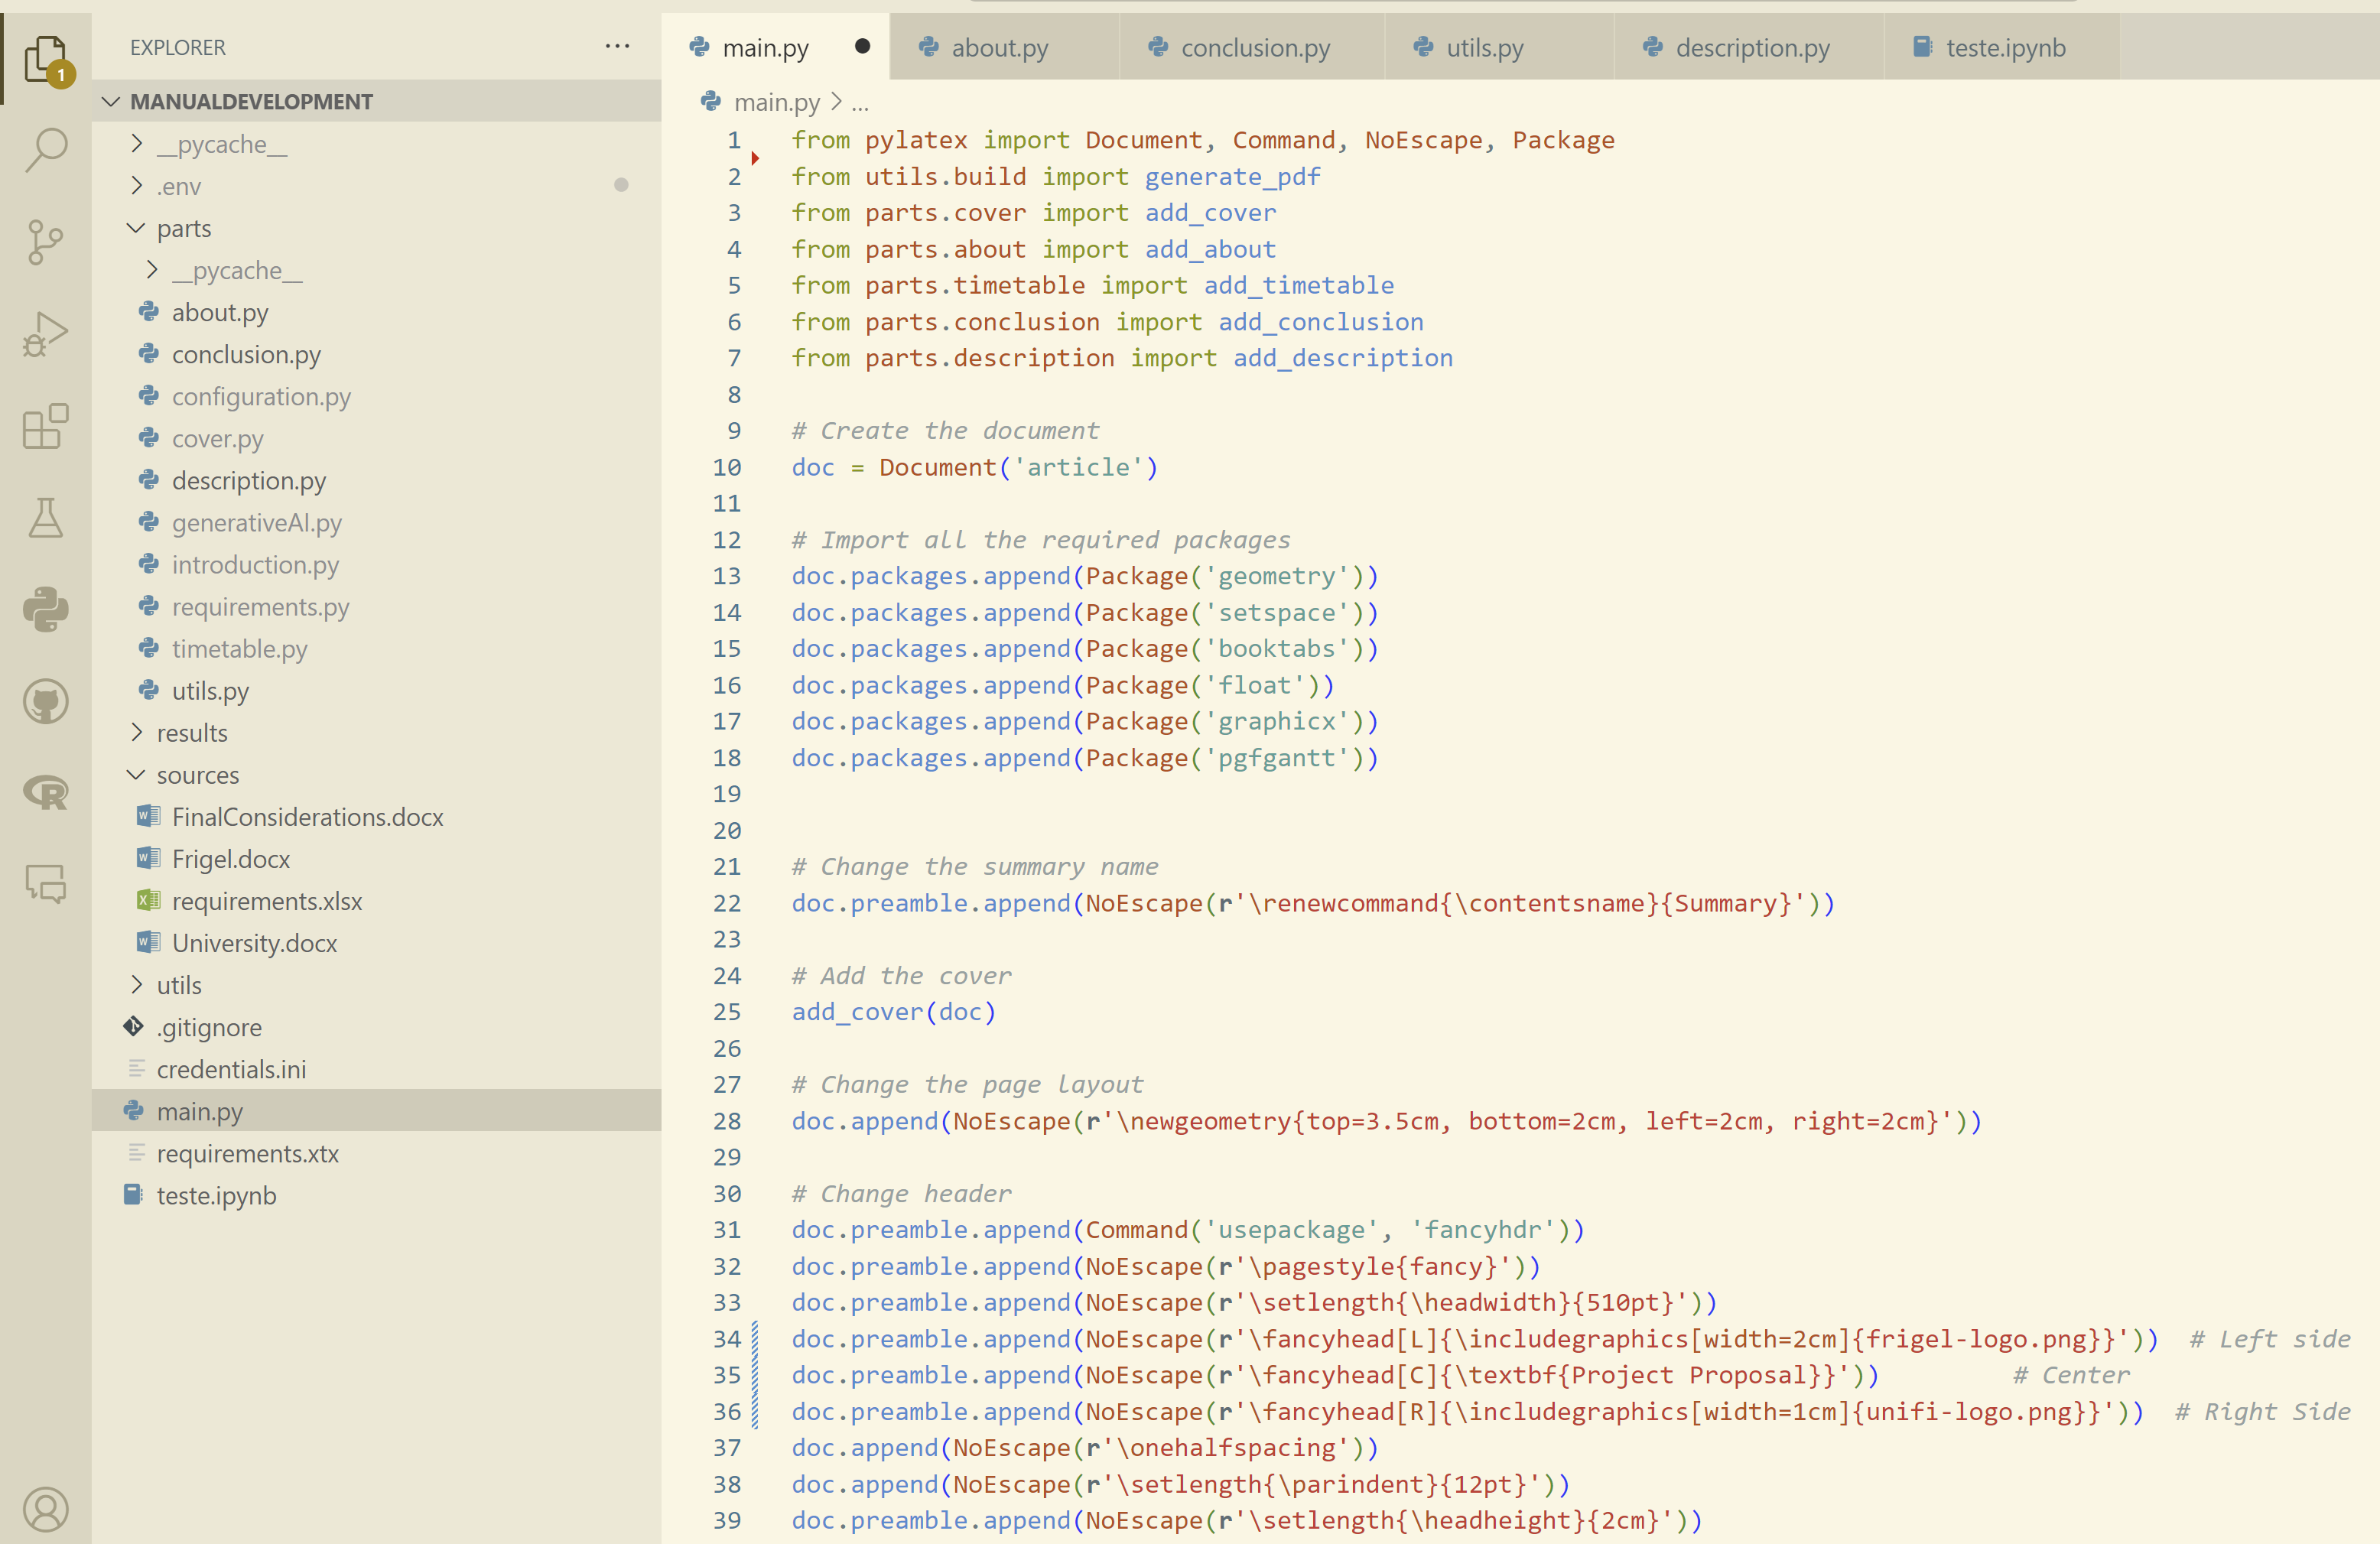
\includegraphics[width=0.8\textwidth]{images/doc1/image1.jpeg}
\end{figure}

Frigel's mission is to engineer more efficient and sustainable industrial processes. Their vision is to be a global innovator in high-performance, sustainable, and quality-engineered solutions for process cooling and temperature control technologies. By focusing on productivity, efficiency, sustainability, and reliability, Frigel aims to meet the evolving needs of industries worldwide.

\begin{figure}[H]
\centering
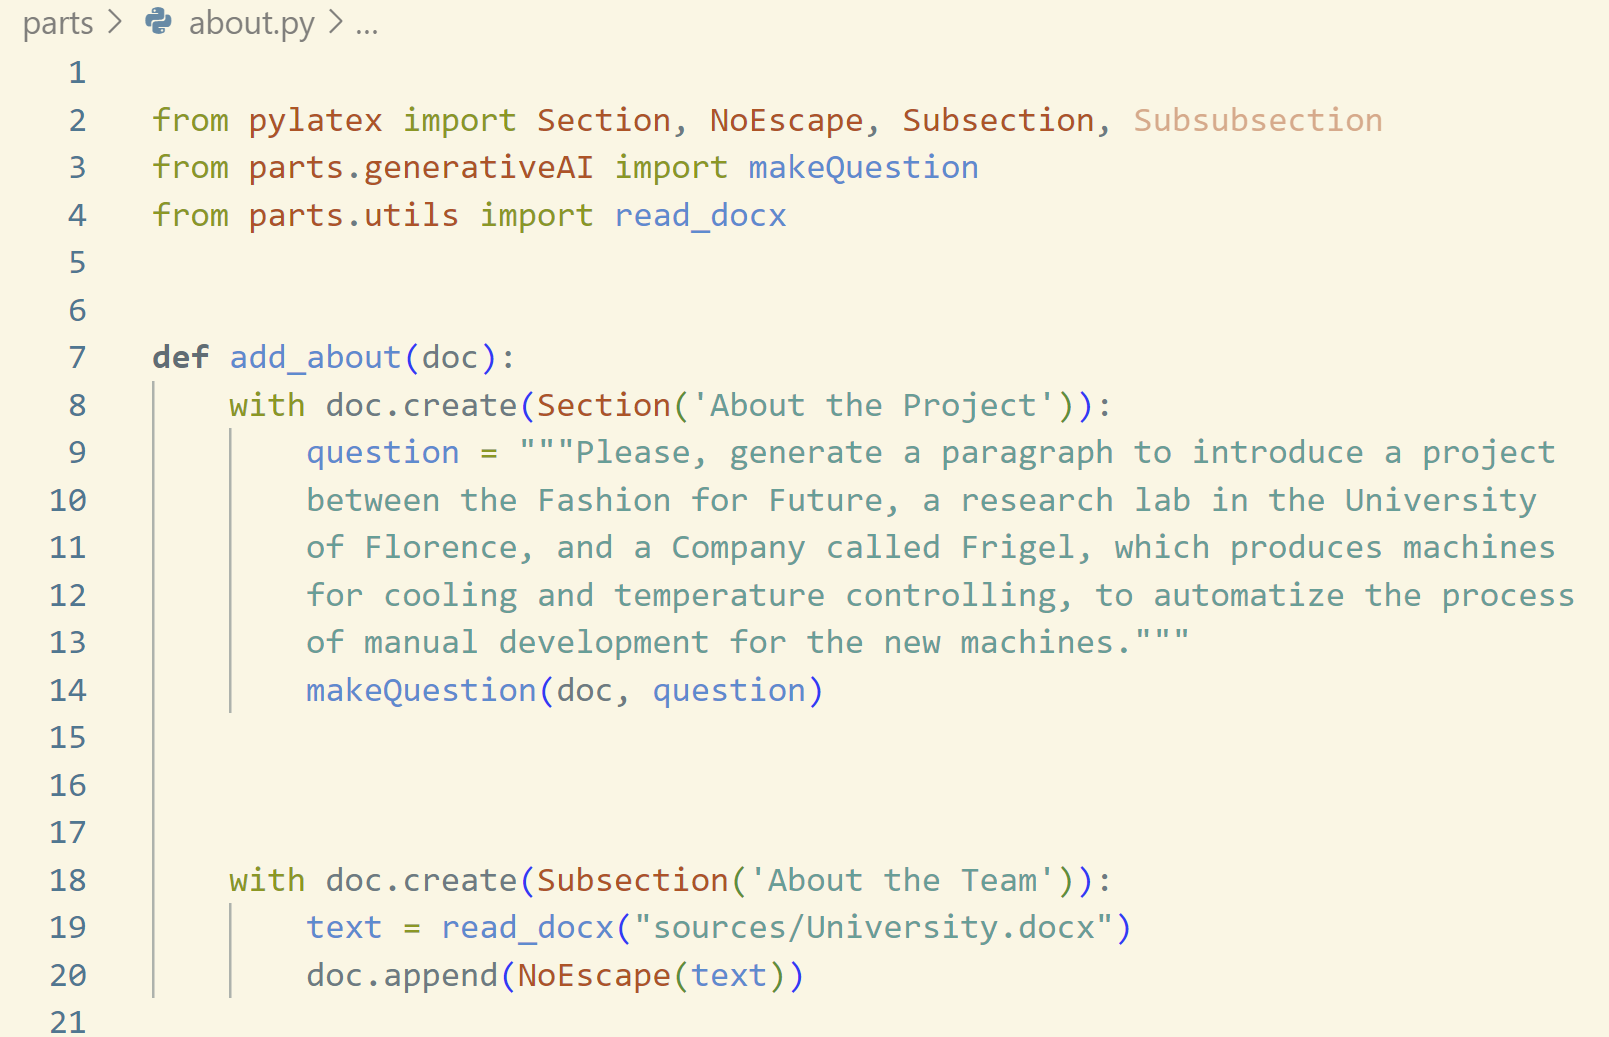
\includegraphics[width=0.8\textwidth]{images/doc1/image2.jpeg}
\end{figure}

TEXTO 3

\begin{figure}[H]
\centering
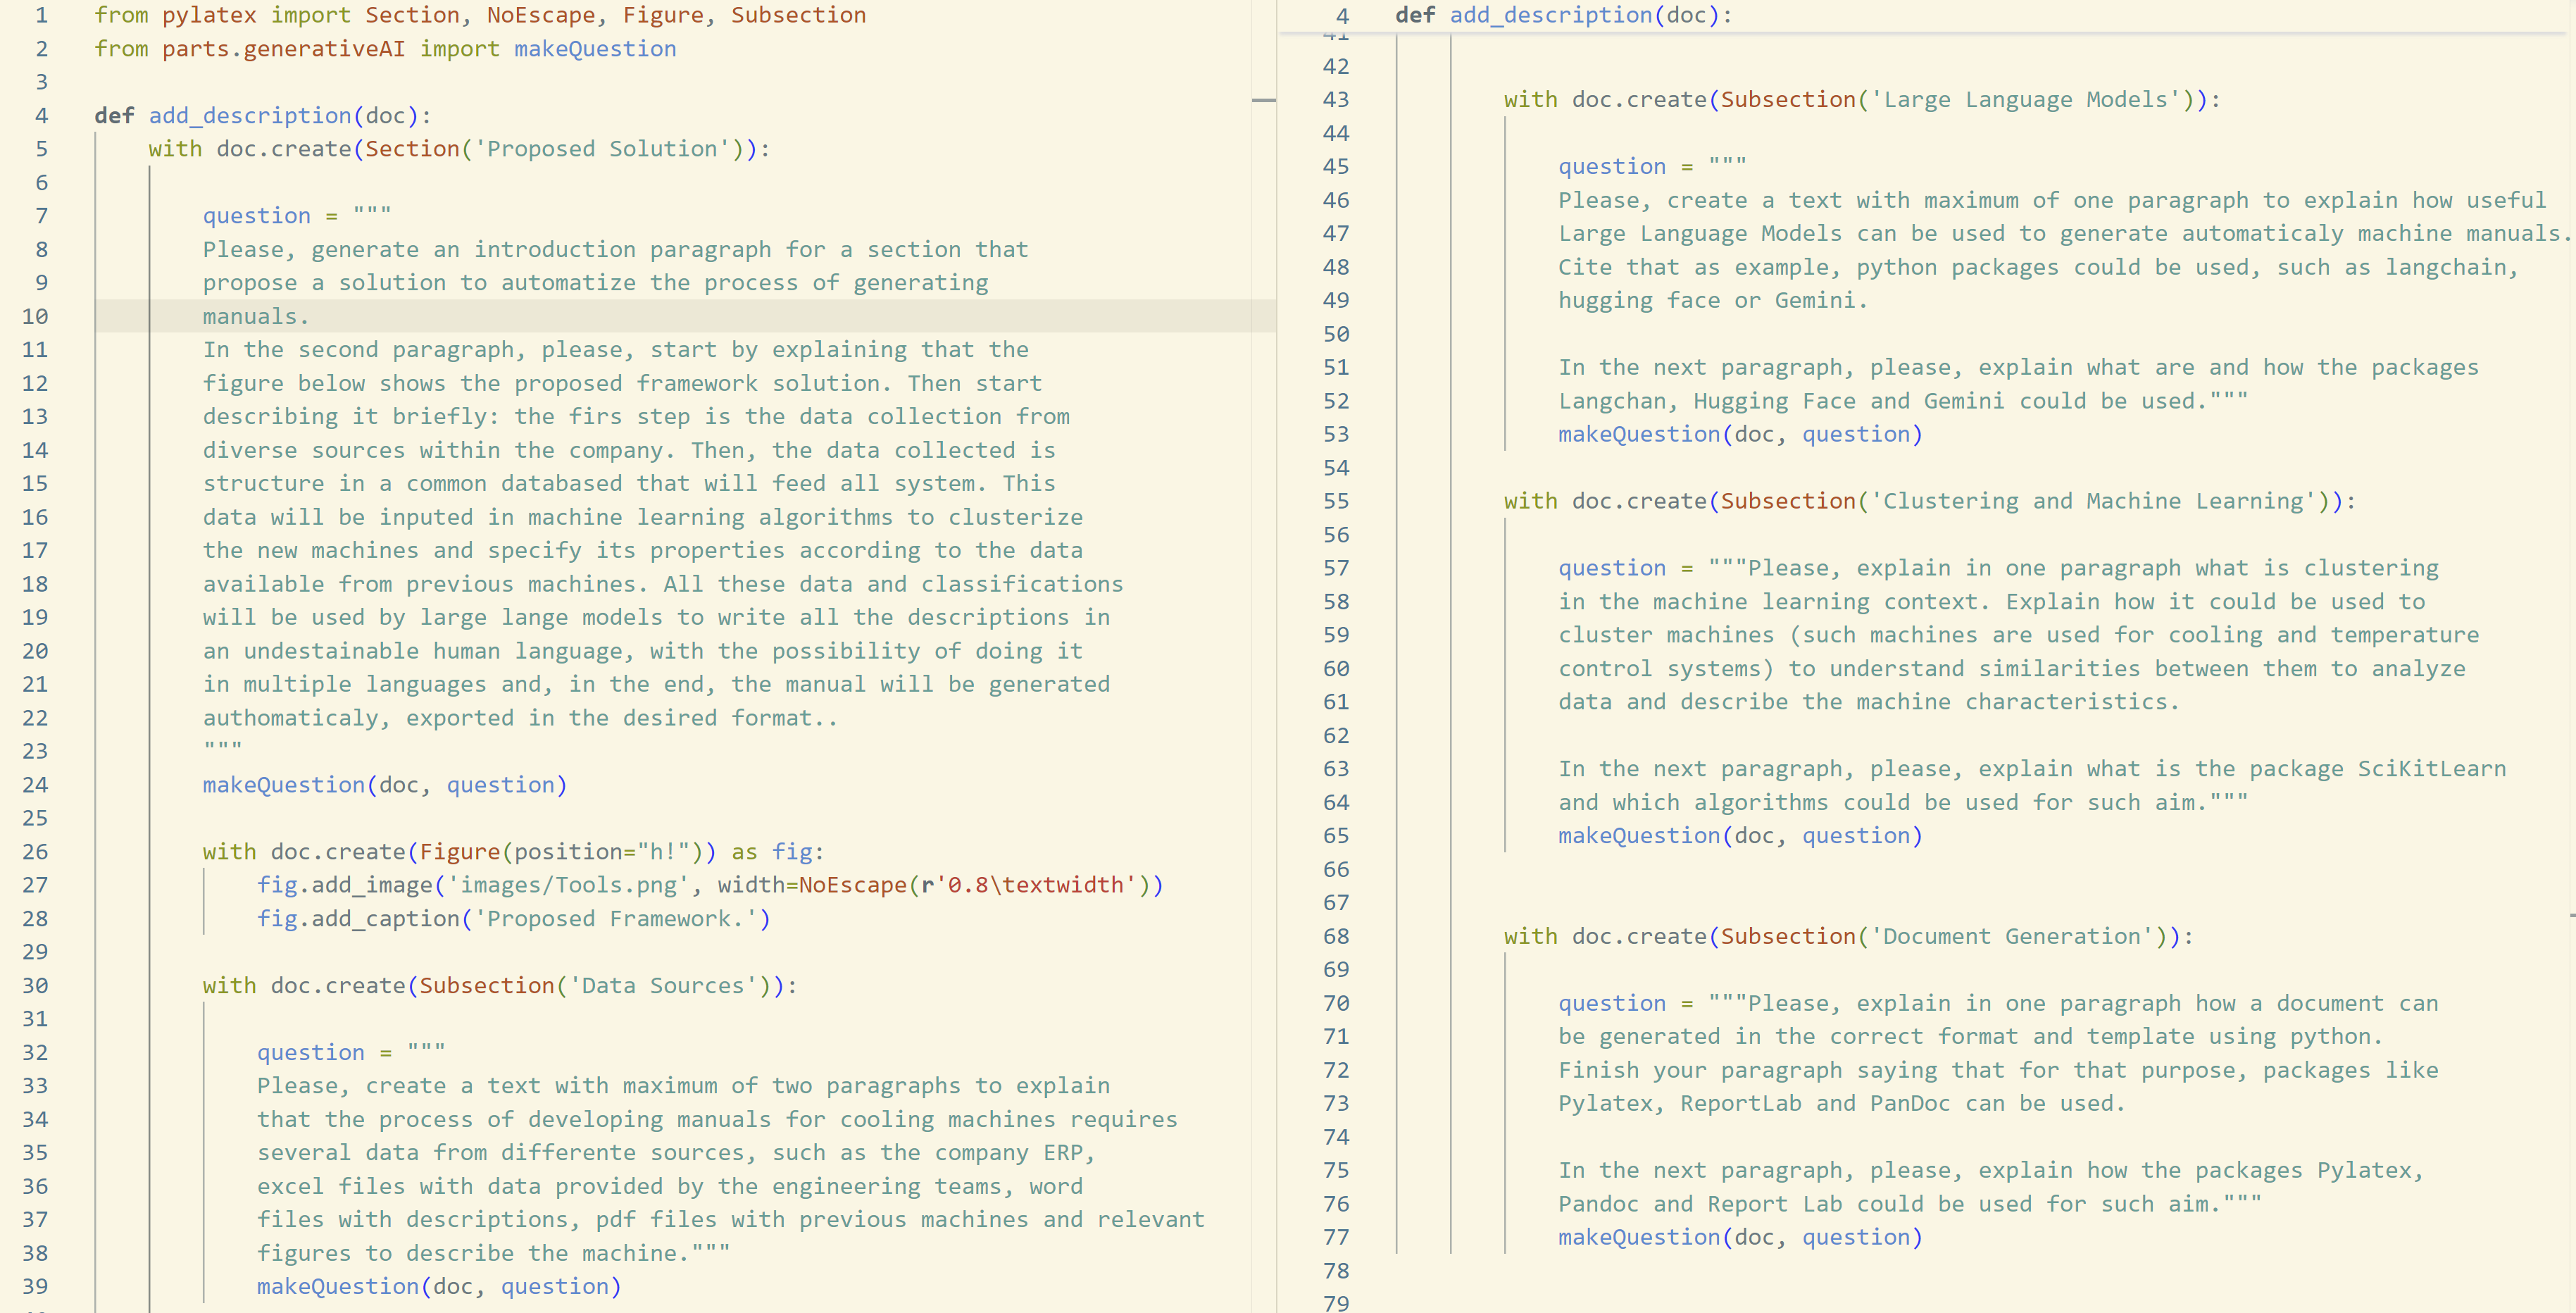
\includegraphics[width=0.8\textwidth]{images/doc1/image3.jpeg}
\end{figure}

TEXTO 4

\begin{figure}[H]
\centering
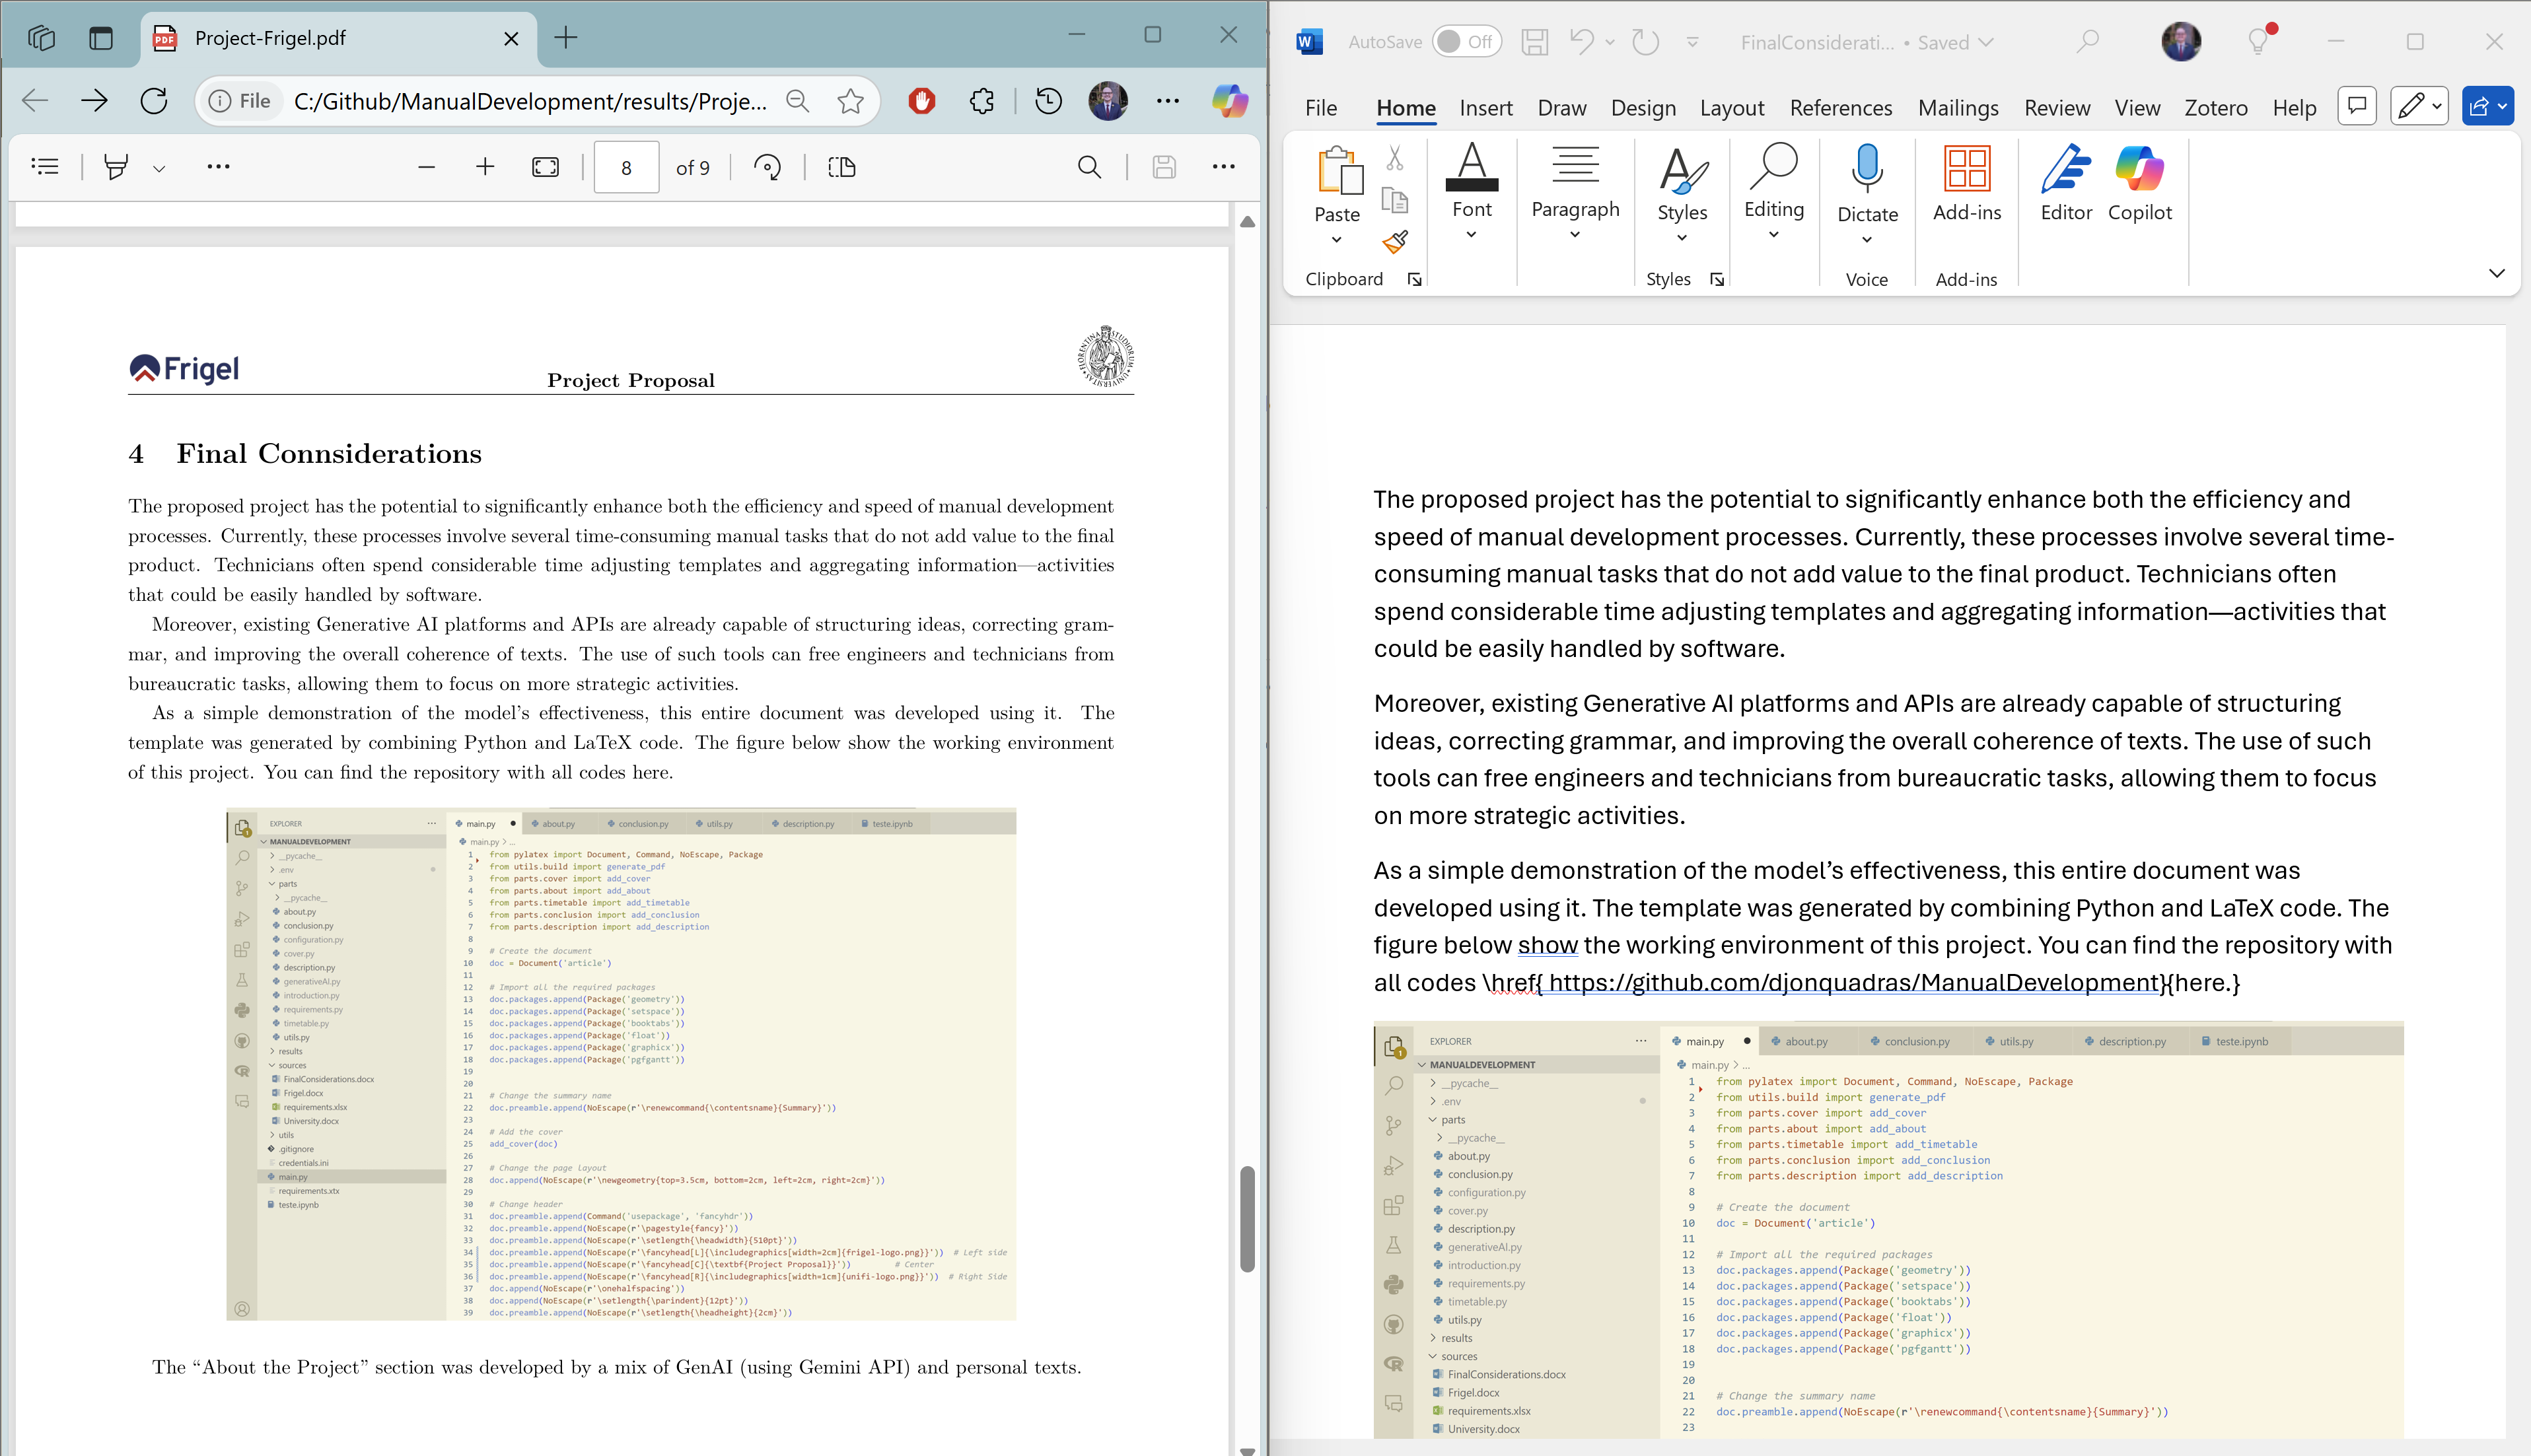
\includegraphics[width=0.8\textwidth]{images/doc1/image4.jpeg}
\end{figure}

%
\end{document}